\documentclass[border=1cm,10pt]{standalone}

% I only need the arrows for this one.
\usepackage{tikz}
\usetikzlibrary{arrows}
\usetikzlibrary{decorations.pathmorphing}
\usetikzlibrary{decorations.markings}
\usetikzlibrary{trees}

\usepackage{nicefrac}

\begin{document}

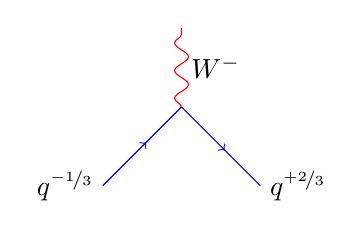
\begin{tikzpicture}[
  boson/.style={decorate, decoration={snake}, draw=red},
  lepton/.style={draw=blue, postaction={decorate},
        decoration={markings,mark=at position .55 with {\arrow[draw=blue]{>}}}},
  alepton/.style={draw=blue, postaction={decorate},
        decoration={markings,mark=at position .55 with {\arrow[draw=blue]{<}}}},
  quark/.style={draw=black, postaction={decorate},
        decoration={markings,mark=at position .55 with {\arrow[draw=black]{>}}}},
  aquark/.style={draw=black, postaction={decorate},
        decoration={markings,mark=at position .55 with {\arrow[draw=black]{<}}}},
]

% Draw the fermions
\draw[lepton] (0,0) node[left] {$q^{\nicefrac{-1}{3}}$} -- (1,1) ;
\draw[lepton] (1,1) -- (2,0) node[right] {$q^{\nicefrac{+2}{3}}$} ;

% Draw the boson
\draw[boson] (1,1) -- (1,2) node[midway,right] {$W^{-}$} ;

\end{tikzpicture}

\end{document} 
